\documentclass[12pt,letterpaper]{exam}
\usepackage[lmargin=1in,rmargin=1in,tmargin=1in,bmargin=1in]{geometry}
\usepackage{../style/exams}

% -------------------
% Course & Exam Information
% -------------------
\newcommand{\course}{MAT 307: Exam 3}
\newcommand{\term}{Spring -- 2023}
\newcommand{\examdate}{05/04/2023}
\newcommand{\timelimit}{85 Minutes}

\setbool{hideans}{true} % Student: True; Instructor: False

% -------------------
% Content
% -------------------
\begin{document}

\examtitle
\instructions{Write your name on the appropriate line on the exam cover sheet. This exam contains \numpages\ pages (including this cover page) and \numquestions\ questions. Check that you have every page of the exam. Indicate your answer for each question in the answer column in the table below. You need not indicate your answers for each question both on the cover page and in the subsequent pages. You may show as much or as little work as you would like; however, only the answers on this cover page will be graded. Be sure each answer is legible and in the correct box. Do not write in the `Points' box on this page.} 
%\scores
%\bottomline

\vfill

\begin{table}[!ht]
\centering
\begin{tabular}{|
>{\columncolor[HTML]{C0C0C0}}c |c|
>{\columncolor[HTML]{C0C0C0}}c |c|
>{\columncolor[HTML]{C0C0C0}}c |c|}
\hline
\cellcolor[HTML]{000000}{\color[HTML]{FFFFFF} \textbf{Question}} & \cellcolor[HTML]{000000}{\color[HTML]{FFFFFF} \textbf{Answer}} & \cellcolor[HTML]{000000}{\color[HTML]{FFFFFF} \textbf{Question}} & \cellcolor[HTML]{000000}{\color[HTML]{FFFFFF} \textbf{Answer}} & \cellcolor[HTML]{000000}{\color[HTML]{FFFFFF} \textbf{Question}} & \cellcolor[HTML]{000000}{\color[HTML]{FFFFFF} \textbf{Answer}} \\ \hline
1 &  & 11 &  & 21 &  \\ \hline
2 &  & 12 &  & 22 &  \\ \hline
3 &  & 13 &  & 23 &  \\ \hline
4 &  & 14 &  & 24 &  \\ \hline
5 &  & 15 &  & 25 &  \\ \hline
6 &  & 16 &  & 26 &  \\ \hline
7 &  & 17 &  & 27 &  \\ \hline
8 &  & 18 &  & 28 &  \\ \hline
9 &  & 19 &  & 29 &  \\ \hline
10 &  & 20 &  & 30 &  \\ \hline
\end{tabular}
\end{table}

\vspace{0.5cm}

	\begin{table}[!ht]
	\centering
	\begin{tabular}{|c|c|} \hline 
	\rowcolor[HTML]{000000} 
	{\color[HTML]{FFFFFF} Points} & {\color[HTML]{FFFFFF} Total} \\ \hline
	& 30 \\ \hline
	\end{tabular}
	\end{table}

\vspace{3cm}
\vfill

\newpage


% ---------
% Questions
% ---------
\begin{questions}

% Question 1
\question Which of the following cannot be the lengths of the sides of a triangle?
	\begin{enumerate}[(a)]
	\item $1$, $7$, $8$
	\item $7$, $8$, $9$
	\item $5$, $26$, $30$
	\item $19$, $180$, $181$
	\end{enumerate} \vfill



% Question 2
\question If $\Delta ABC$ is a right triangle whose shortest side has length $12$ and whose longest side is $37$, what is the length of the other side of the triangle? 
	\begin{enumerate}[(a)]
	\item $12.25$
	\item $24.5$
	\item $25$
	\item $35$
	\end{enumerate} \vfill



% Question 3
\question Suppose a triangle has sides with length 85 and 112. What is the smallest possible length of the third side if the side must have a length which is an integer? 
	\begin{enumerate}[(a)]
	\item $27$
	\item $28$
	\item $197$
	\item $198$
	\end{enumerate} \vfill



% Question 4
\question Triangle $\Delta ABC$ is a right triangle with side lengths $20$, $21$, and $29$. We know that the shortest side of $\Delta DEF$ has length 5 and $\Delta DEF \sim \Delta ABC$. What is the area of $\Delta DEF$?
	\begin{enumerate}[(a)]
	\item $13.1$
	\item $52.5$
	\item $70.0$
	\item $210.0$
	\end{enumerate} \vfill



\newpage



% Question 5
\question Find $x$ in the triangle below. 
	\[
	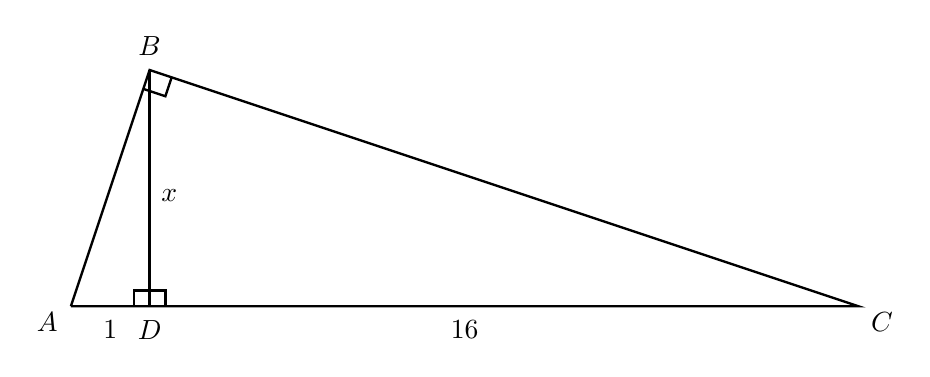
\begin{tikzpicture}
	\draw[line width=0.03cm] (0,0) -- (1,3) -- (10,0) -- (0,0);
	\draw[line width=0.03cm] (1,3) -- (1,0);
	\draw[line width=0.03cm] (0.8,0) -- (0.8,0.2) -- (1.2,0.2) -- (1.2,0);
	\draw[line width=0.03cm] (0.92,2.76) -- (1.2,2.666) -- (1.2802,2.9066);
	\node at (-0.3,-0.2) {$A$};
	\node at (1,3.3) {$B$};
	\node at (10.3,-0.2) {$C$};
	\node at (1,-0.3) {$D$};
	\node at (0.5,-0.3) {$1$};
	\node at (1.25,1.4) {$x$};
	\node at (5,-0.3) {$16$};
	\end{tikzpicture}
	\] 

\begin{enumerate}[(a)]
\item $1$
\item $4$
\item $8$
\item $10$
\end{enumerate} \vfill



% Question 6
\question Which of the following geometric constructions is not possible using a straightedge and compass?
	\begin{enumerate}[(a)]
	\item Constructing a perpendicular bisector to a given line segment. 
	\item Constructing an angle double the measure of a given angle. 
	\item Constructing the angle bisector of a given angle. 
	\item Constructing the angle trisector of a given angle. 
	\end{enumerate} \vfill



% Question 7
\question Suppose a regular octagonal cylinder has volume $165.3$~cm$^3$. What is the volume of the cylinder after a dilation with scale factor $2.5$?
	\begin{enumerate}[(a)]
	\item $10.58$~cm$^3$
	\item $66.12$~cm$^3$
	\item $413.25$~cm$^3$
	\item $2582.81$~cm$^3$
	\end{enumerate} \vfill



% Question 8
\question Which of the following properties does not guarantee that two triangles are congruent?
	\begin{enumerate}[(a)]
	\item AAA
	\item SSS
	\item SAS
	\item AAS
	\end{enumerate} \vfill



\newpage



% Question 9
\question Which of the following is \textit{not} true. 
	\begin{enumerate}[(a)]
	\item The plane can be tiled with \textit{any} triangular tile. 
	\item The plane can be tiled with \textit{any} quadrilateral tile. 
	\item The plane can be tiled with \textit{any} pentagonal tile. 
	\item The plane can be tiled with \textit{some} hexagonal tiles. 
	\end{enumerate} \vfill



% Question 10
\question What is the measure of the largest angle in an isosceles triangle whose smallest angle is $12^\circ$?
	\begin{enumerate}[(a)]
	\item $12^\circ$
	\item $84^\circ$
	\item $156^\circ$
	\item $168^\circ$
	\end{enumerate} \vfill



% Question 11
\question Suppose you are given three distinct positive integers $a$, $b$, and $c$. What is maximum number of distinct triangles with sides having length $a$, $b$, and $c$ that can be constructed?
	\begin{enumerate}[(a)]
	\item $0$
	\item $1$
	\item $2$
	\item $3$
	\end{enumerate} \vfill



% Question 12
\question Suppose you are given three distinct positive integers $a$, $b$, and $c$. How many distinct triangles with angles having measures $a$, $b$, and $c$ can be constructed? 
	\begin{enumerate}[(a)]
	\item $0$
	\item $1$
	\item $3$
	\item Infinitely many
	\end{enumerate} \vfill



% Question 13
\question How many distinct right triangles are with the hypotenuse having length $13$ if the hypotenuse makes angles $56^\circ$ and $64^\circ$ with the legs of the triangle?
	\begin{enumerate}[(a)]
	\item $0$
	\item $1$
	\item $3$
	\item Infinitely many 
	\end{enumerate} \vfill



\newpage



% Question 14
\question Which of the following cannot be used to regularly tile the plane?
	\begin{enumerate}[(a)]
	\item equilateral triangles
	\item squares
	\item regular pentagons
	\item regular hexagons
	\end{enumerate} \vfill



% Question 15
\question Which of the following statements is \textit{not} true?
	\begin{enumerate}[(a)]
	\item All congruent triangles are similar. 
	\item All similar triangles are congruent. 
	\item The image of a triangle under a glide reflection is always congruent to the preimage. 
	\item The image of a triangle under a dilation is always similar to the preimage. 
	\end{enumerate} \vfill



% Question 16
\question Suppose that $\Delta ABC$ is a right triangle with sides $33$, $56$, and $65$, and $\Delta ABC \sim \Delta DEF$. If the hypotenuse of $\Delta DEF$ has length $260$, find the length of the shortest side of $\Delta DEF$.
	\begin{enumerate}[(a)]
	\item $14$
	\item $16$
	\item $132$
	\item $224$
	\end{enumerate} \vfill



% Question 17
\question Suppose that $\Delta ABC$ is a right triangle and $\Delta ABC \sim \Delta DEF$. If $|\overline{AB}| = |\overline{BC}|$, which of the following is the measure of the smallest angle in $\Delta DEF$.
	\begin{enumerate}[(a)]
	\item $30^\circ$
	\item $45^\circ$
	\item $50^\circ$
	\item $60^\circ$
	\end{enumerate} \vfill



% Question 18
\question Suppose that $\Delta ABC \cong \Delta DEF$. If $\Delta ABC$ is isosceles, which of the following is \textit{not} true about $\Delta DEF$:
	\begin{enumerate}[(a)]
	\item $\Delta DEF$ is isosceles. 
	\item $\Delta DEF$ is a right triangle.
	\item $\Delta DEF$ has two congruent angles. 
	\item $\Delta DEF$ is similar to $\Delta ABC$.
	\end{enumerate} \vfill



\newpage



% Question 19
\question The sides of a right triangle with angles $30^\circ$, $60^\circ$, and $90^\circ$ are in the proportion $1 \colon \sqrt{3} \colon 2$. If the hypotenuse of $30^\circ$, $60^\circ$, $90^\circ$ triangle has length $10.87$, what is the length of the second largest side?
	\begin{enumerate}[(a)]
	\item $5.44$
	\item $6.28$
	\item $9.41$
	\item $12.55$
	\end{enumerate} \vfill



% Question 20
\question Which of the following is \textit{not} a rigid transformation?
	\begin{enumerate}[(a)]
	\item translation
	\item reflection
	\item dilation
	\item rotation 	
	\end{enumerate} \vfill



% Question 21
\question If the two horizontal lines shown below are parallel, find $x$.
	\[
	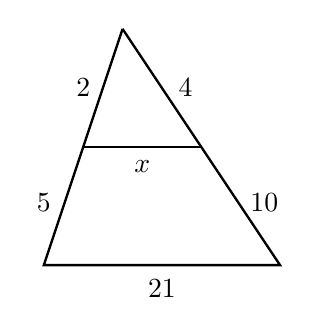
\begin{tikzpicture}
	\draw[line width=0.03cm] (0,3) -- (-1,0) -- (2,0) -- (0,3);
	\draw[line width=0.03cm] (-0.5,1.5) -- (1,1.5);
	\node at (0.25,1.25) {$x$};
	\node at (0.5,-0.3) {$21$};
	\node at (-0.5,2.25) {$2$};
	\node at (0.8,2.25) {$4$};
	\node at (-1,0.8) {$5$};

	\node at (1.8,0.8) {$10$};
	\end{tikzpicture}
	\]

\begin{enumerate}[(a)]
\item $6$
\item $8$
\item $10$
\item $12$
\end{enumerate} \vfill



% Question 22
\question If the image of reflecting a point $P$ through the line $x= 2$ is $(-4, 6)$, which of the following is $P$?
	\begin{enumerate}[(a)]
	\item $(2, 6)$
	\item $(8, 6)$
	\item $(-6, 6)$
	\item $(6, -4)$
	\end{enumerate} \vfill



\newpage



% Question 23
\question Which of the following is the image of the point $P= (5, -2)$ after a rotation of $90^\circ$ counterclockwise about the origin?
	\begin{enumerate}[(a)]
	\item $(-5, -2)$
	\item $(-2, 5)$
	\item $(2, 5)$
	\item $(5, 2)$
	\end{enumerate} \vfill



% Question 24
\question Suppose that $a < b$. If one reflects a point $P$ through the line $x= a$ and then reflects the image through the line $x= b$, which of the following is an equivalent transformation? 
	\begin{enumerate}[(a)]
	\item A translation of $P$ a distance $2(a + b)$ to the right. 
	\item A translation of $P$ a distance $2(b - a)$ to the left. 
	\item A translation of $P$ a distance $2(a + b)$ to the left.  
	\item A translation of $P$ a distance $2(b - a)$ to the right. 
	\end{enumerate} \vfill
	


% Question 25
\question Suppose one reflects a point $P$ through the line $x= 2$ and then reflects this image through the line $y= 3$. Which of the following is an equivalent transformation?
	\begin{enumerate}[(a)]
	\item A rotation of $180^\circ$ about the point $(2, 3)$
	\item A translation of 2 to the right and 3 upwards.
	\item A rotation of $180^\circ$ about the origin. 
	\item A translation of 2 to the left and 3 downwards. 
	\end{enumerate} \vfill



% Question 26
\question Which of the following transformations is a rigid transformation which does \textit{not} preserve orientation?
	\begin{enumerate}[(a)]
	\item dilation
	\item  translation 
	\item rotation 
	\item reflection 	
	\end{enumerate} \vfill



\newpage



% Question 27
\question A regular decagon has sides with length $17.9$~m. After a dilation with scale factor $0.6$, what is the perimeter of the resulting decagon?
	\begin{enumerate}[(a)]
	\item $10.74$~m
	\item $23.9$~m
	\item $107.4$~m
	\item $185$~m
	\end{enumerate} \vfill



% Question 28
\question Let $T$ be the translation of a point $(x, y)$ given by $(x - 3, y + 2)$. Let $T'$ be the translation of a point $(x, y)$ given by $(x + 6, y - 3)$. Let $P$ be the image of the point $(x, y)$ after applying the transformation $T$ and then $T'$. Which of the following is the translation that take the point $P$ to the point $(x, y)$?
	\begin{enumerate}[(a)]
	\item $(x + 3, y - 1)$
	\item $(x + 9, y - 5)$
	\item $(y - 3, x + 1)$
	\item $(x - 3, y + 1)$
	\end{enumerate} \vfill



% Question 29
\question Find $x$ in the triangle below. 
	\[
	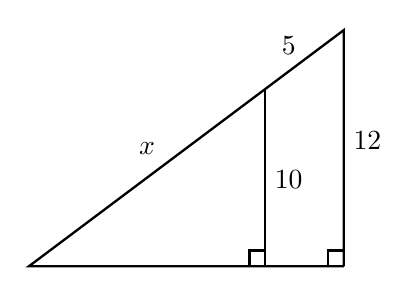
\begin{tikzpicture}
	\draw[line width=0.03cm] (0,0) -- (0,3) -- (-4,0) -- (0,0);
	\draw[line width=0.03cm] (-1,0) -- (-1,2.25);
	\draw[line width=0.03cm] (0,0.2) -- (-0.2,0.2) -- (-0.2,0);
	\draw[line width=0.03cm] (-1,0.2) -- (-1.2,0.2) -- (-1.2,0);
	\node at (0.3,1.6) {$12$};
	\node at (-0.7,1.1) {$10$};
	\node at (-0.7,2.8) {$5$};
	\node at (-2.5,1.5) {$x$};
	\end{tikzpicture}
	\]

\begin{enumerate}[(a)]
\item $3$
\item $6$
\item $25$
\item $27$
\end{enumerate} \vfill



% Question 30
\question Which of the following regular $n$-gon is \textit{not} constructible with a compass and straightedge?
	\begin{enumerate}[(a)]
	\item $3$-gon
	\item $4$-gon
	\item $5$-gon
	\item $9$-gon
	\end{enumerate} \vfill


\end{questions}
\end{document}